\documentclass[10pt,twoside,openright]{book}

% Essential packages
\usepackage[utf8]{inputenc}
\usepackage[T1]{fontenc}
\usepackage{lmodern}
\usepackage{microtype}
\usepackage[english]{babel}

% Japanese/CJK support for pdfLaTeX
\usepackage{CJKutf8}
\newcommand{\ja}[1]{\begin{CJK}{UTF8}{min}#1\end{CJK}} % Helper command for Japanese text

% Page layout
\usepackage[
    paperwidth=6in,
    paperheight=9in,
    top=0.75in,      % Reduced from 1in
    bottom=0.75in,   % Reduced from 1in
    inner=1in,       % Reduced from 1.25in
    outer=0.6in      % Reduced from 0.75in
]{geometry}

% Typography and formatting
\usepackage{setspace}
\singlespacing  % Changed from onehalfspacing to reduce size
\usepackage{parskip}
\setlength{\parindent}{0pt}
\setlength{\parskip}{0.3\baselineskip}  % Reduced from 0.5

% Graphics and tables
\usepackage{graphicx}
\usepackage{booktabs}
\usepackage{longtable}
\usepackage{array}
\usepackage{multirow}
\usepackage{float}
\usepackage{caption}
\usepackage{subcaption}

% Reduce spacing around floats
\setlength{\floatsep}{10pt plus 2pt minus 2pt}
\setlength{\textfloatsep}{10pt plus 2pt minus 2pt}
\setlength{\intextsep}{10pt plus 2pt minus 2pt}
\setlength{\abovecaptionskip}{5pt}
\setlength{\belowcaptionskip}{5pt}

% Math and statistics
\usepackage{amsmath}
\usepackage{amssymb}
\usepackage{amsthm}

% Bibliography
\usepackage[backend=biber,style=numeric,natbib=true]{biblatex}
\addbibresource{src/references.bib}
% Use superscript citations
\DeclareCiteCommand{\cite}
  {\usebibmacro{prenote}}
  {\usebibmacro{citeindex}%
   \textsuperscript{\usebibmacro{cite}}}
  {\multicitedelim}
  {\usebibmacro{postnote}}

% Hyperlinks
\usepackage[colorlinks=true,linkcolor=black,urlcolor=blue,citecolor=black]{hyperref}

% Code listings
\usepackage{listings}
\lstset{
    basicstyle=\ttfamily\small,
    breaklines=true,
    frame=single
}

% Custom commands
\newcommand{\japterm}[2]{#1 (\ja{#2})}  % Now supports kanji in the second argument
\newcommand{\kimarite}[1]{\textit{#1}}

% Index
\usepackage{makeidx}
\makeindex

% Chapter and section styling
\usepackage{titlesec}
\titleformat{\chapter}[display]
{\normalfont\huge\bfseries}
{\chaptertitlename\ \thechapter}
{10pt}  % Reduced from 20pt
{\Huge}
\titlespacing*{\chapter}{0pt}{-30pt}{20pt}  % Reduce space before/after chapters

% Section spacing - reduced spacing (original)
\titlespacing*{\section}{0pt}{3.5ex plus 1ex minus .2ex}{2.3ex plus .2ex}
\titlespacing*{\subsection}{0pt}{3.25ex plus 1ex minus .2ex}{1.5ex plus .2ex}
\titlespacing*{\subsubsection}{0pt}{3ex plus 1ex minus .2ex}{1.5ex plus .2ex}

% Table of Contents spacing - clean, structured hierarchy
\usepackage{tocloft}
% Section spacing
\setlength{\cftsecnumwidth}{2.8em}        % Width for section numbers
\setlength{\cftsecindent}{0em}            % No indent for sections
\setlength{\cftbeforesecskip}{0.3em}      % Small space before sections

% Subsection spacing
\setlength{\cftsubsecnumwidth}{3.5em}     % Width for subsection numbers
\setlength{\cftsubsecindent}{2.8em}       % Indent subsections by section number width
\setlength{\cftbeforesubsecskip}{0.15em}  % Minimal space before subsections

% Subsubsection spacing
\setlength{\cftsubsubsecnumwidth}{4.2em}  % Width for subsubsection numbers
\setlength{\cftsubsubsecindent}{6.3em}    % Indent by section + subsection widths
\setlength{\cftbeforesubsubsecskip}{0.1em} % Minimal space before subsubsections

% Add leader dots for better readability
\renewcommand{\cftsecleader}{\cftdotfill{\cftdotsep}}
\renewcommand{\cftsubsecleader}{\cftdotfill{\cftdotsep}}
\renewcommand{\cftsubsubsecleader}{\cftdotfill{\cftdotsep}}

% Document info
\title{The Science of Sumo: Data, Technique, and Performance in Professional Wrestling}
\author{Joseph Babcanec}
\date{\today}

\begin{document}

% Front matter
\frontmatter
\maketitle

\tableofcontents

\clearpage
\listoffigures

\clearpage
\listoftables

% Preface
\chapter*{Preface: How to Read This Book}
\addcontentsline{toc}{chapter}{Preface}

\section*{A Personal Note}

My interest in sumo began in early 2025, though my fascination with Japanese culture extends back years. I'd studied Japanese orthography, practiced kendo briefly, absorbed the language and aesthetics of a culture that seemed to have mastered something I found compelling: the ability to codify chaos into defined, almost artistic practice. Japan takes the messiness of human activity—whether it's brewing tea, arranging flowers, or two massive men trying to throw each other out of a ring—and transforms it into something with clear rules, deep tradition, and profound meaning.

I remember reading on Japanese Wikipedia about Hoshoryu's promotion to yokozuna and wanting to understand more. The stable system intrigued me—young men living communally under brutal hierarchical structures, dedicating their lives to mastering a sport most would never succeed in. The evolution of sumo as a cultural landmark, surviving wars and modernization while maintaining rituals over a millennium old, felt like a case study in how tradition and change negotiate with each other.

But what really hooked me was the simplicity. You can understand sumo in seconds just by watching one match. The rules are clear: force your opponent out of the circle or make any part of their body besides their feet touch the ground. That's it. Yet within that simplicity exists extraordinary complexity—technique, strategy, psychology, physical conditioning. This combination of accessible surface and deep structure is characteristic of what I admire about Japanese cultural forms.

I began this book because I'm interested in statistical ramifications. American baseball recruiting has become a game of which team employs the better mathematician. Basketball analysts can predict success using hand size or seemingly arbitrary physical measurements. I wanted to explore whether similar approaches could work for sumo, and what unique statistical phenomena might emerge from a sport with such different institutional structures than Western professional athletics.

I should be transparent about methodology: I use AI extensively in writing this book. This reflects a practical division of labor based on my actual interests and skills. I design and perform all statistical analysis myself—the models, the data processing, the interpretation of results. That's what I care about and what I'm trained to do. For contextual material like historical background, I guide the subject matter and structure, but I'm not precious about writing my own version of historical facts that have been documented elsewhere. AI handles synthesis of that existing knowledge efficiently, freeing me to focus on original analytical work. The history chapter you're reading? AI-generated from primary and secondary sources, under my direction. The statistical models in later chapters? Those are mine, along with the interpretations and implications.

This isn't laziness; it's honest allocation of effort toward what I can contribute uniquely. I'm not a historian of Japanese culture or an expert on Shinto ritual. But I can build regression models, evaluate predictive accuracy, and think carefully about causal inference in observational data. That's where this book's value lies, and that's where I've invested my time.

\section*{Research Questions}

Sumo wrestling, Japan's ancient national sport, stands at a fascinating intersection of tradition and evolution. While the rituals and cultural significance remain unchanged across centuries, the athletes, techniques, and competitive dynamics have undergone remarkable transformations. This book asks fundamental questions about that evolution: What factors truly influence success in the ring? Can we identify patterns that predict future performance? How do training practices, body composition, and technique selection evolve over time in response to competitive pressures?

Modern American sports analytics has revolutionized how we understand athletic performance---from baseball's sabermetrics to basketball's spatial tracking, teams now leverage sophisticated statistical models to evaluate talent, predict outcomes, and optimize strategies. A central question driving this work is whether these same analytical frameworks can illuminate sumo wrestling, a sport with fundamentally different structure, constraints, and cultural context. Can we build rating systems that capture wrestler quality beyond win-loss records? Can injury risk be predicted and mitigated? What recruiting characteristics signal future yokozuna potential?

This investigation reveals both universal patterns that transcend sporting contexts and unique dynamics specific to sumo's institutional structure. The same statistical tools that evaluate NBA draft prospects can identify promising young rikishi, yet sumo's stable system, foreign-born wrestler caps, and rigid ranking hierarchy create analytical challenges absent from Western professional sports.

\section*{Purpose and Scope}

This book represents a comprehensive quantitative analysis of professional sumo wrestling, leveraging modern data science techniques to understand the sport's competitive dynamics, strategic elements, and physical demands. Our approach combines rigorous statistical modeling with domain expertise to illuminate patterns that have shaped sumo from 1958 to the present day.

The scope encompasses:
\begin{itemize}
\item Systematic analysis of bout outcomes using mixed-effects models
\item Technique ecology and strategic diversity across eras
\item Physical anthropometry and its relationship to success
\item Injury patterns and career longevity
\item Rating systems and predictive modeling
\item Natural experiments from policy changes
\end{itemize}

\section*{Data Sources and Reproducibility}

All analyses in this book are built on publicly available data sources, primarily:

\begin{itemize}
\item \textbf{Sumo-API}: Primary structured data source (1958--present) providing rikishi profiles, tournament results, banzuke rankings, and bout outcomes
\item \textbf{Japan Sumo Association (JSA)}: Official records for verification and supplementary information
\item \textbf{SumoDB}: Historical cross-validation and extended queries
\item \textbf{Medical Literature}: PubMed and PMC databases for injury prevalence and health outcomes
\end{itemize}

Complete code for data acquisition, processing, and analysis is available at our GitHub repository. All random seeds are fixed for reproducibility, and data snapshots are versioned to ensure consistency across analyses.

\section*{What ``Causality'' Does Not Mean Here}

This book operates primarily in the realm of observational data analysis. When we discuss relationships between variables---such as the association between technique diversity and win rates---we are describing correlations and predictive patterns, not necessarily causal mechanisms.

True causal inference requires either:
\begin{itemize}
\item Randomized controlled experiments (impossible in professional sports)
\item Natural experiments with credible identification strategies
\item Strong theoretical assumptions that may not hold
\end{itemize}

We employ quasi-experimental methods where possible, particularly around policy changes like:
\begin{itemize}
\item The 2003 abolition of the \japterm{kōshō}{kosho} system (injury leave)
\item The 2010 clarification of foreign-born wrestler quotas
\item Changes in tournament frequency and structure
\end{itemize}

However, readers should interpret findings as associations and patterns rather than definitive causal relationships unless explicitly noted otherwise.

\section*{Structural Constraints Shaping the Data}

Several institutional features of professional sumo create unique data-generating processes:

\paragraph{Foreign-Born Wrestler Cap} Each stable (\japterm{heya}{heya}) may have only one foreign-born wrestler at a time. This constraint affects recruitment patterns, career trajectories, and competitive dynamics in ways that must be accounted for in our models.

\paragraph{Same-Stable Non-Competition Rule} Wrestlers from the same stable do not face each other in regular tournament bouts (exceptions exist for playoffs). This creates systematic missing data patterns that affect rating calculations and head-to-head analyses.

\paragraph{Promotion/Demotion System} The rigid ranking system creates discrete jumps in competition level and incentive structures, particularly around the 7-7 record threshold for maintaining rank.

\paragraph{Tournament Structure Evolution} The shift to six tournaments per year in 1958 and other structural changes create era effects that must be controlled for in longitudinal analyses.

\section*{How to Use This Book}

\paragraph{For the General Reader} Focus on Chapters 1--2 for historical context, Chapter 5 for descriptive insights, and Chapter 10 for compelling case studies. Technical sections are clearly marked and can be skipped without losing the narrative thread.

\paragraph{For the Data Scientist} Chapters 3--4 detail our data pipeline and feature engineering. Chapters 6--9 contain the core statistical models. Appendix D provides full model specifications and diagnostic tests.

\paragraph{For the Sumo Enthusiast} Chapter 5's landscape analysis and Chapter 10's case studies will be of particular interest. Appendix B contains a comprehensive kimarite catalog with historical notes.

\paragraph{For Researchers} All data and code are available for replication and extension. We encourage independent verification of our findings and welcome corrections or improvements.

\section*{Acknowledgments}

This work would not have been possible without the meticulous record-keeping of the Japan Sumo Association and the dedication of the sumo data community, particularly the maintainers of Sumo-API and SumoDB.

% Main matter
\mainmatter

% Part I: Foundations
\part{Foundations}
\chapter{A Short History of Sumo}

\section{Origins and Evolution}

Professional sumo wrestling (\japterm{ōzumō}{ozumo}) represents one of the world's oldest continuously practiced sports, with roots extending back over 1,500 years. What began as Shinto harvest rituals evolved through centuries into today's highly structured professional sport, maintaining ceremonial elements while adapting to modern athletic and commercial demands.

The sport's documented history begins in the Nara period (710--794), though archaeological evidence suggests proto-sumo existed centuries earlier. The Nihon Shoki, Japan's second-oldest book of classical history, records a wrestling match in 23 BCE between Nomi no Sukune and Taima no Kuehaya---often cited as sumo's mythological origin.
\section[The Stable System]{The Stable System: Architecture of a Wrestler's World}

If sumo's mythology provided its soul and the Edo period its commercial structure, the \japterm{heya}{部屋} system—literally "room" or "fraternity house"—constitutes its skeleton. Every professional wrestler belongs to a stable, where he lives, trains, eats, and sleeps under the authority of a retired wrestler who shapes not just his technique but his entire existence. The stable is total institution and vocational school, family and factory, all compressed into a hierarchical microcosm that has remained structurally consistent for over two centuries.

Understanding the stable system is essential for any statistical analysis of sumo, because it generates many of the sport's most distinctive patterns. Wrestlers from the same stable never face each other in regular tournament bouts, creating systematic missing data. The foreign-born wrestler cap applies at the stable level, affecting recruitment strategies. Success clusters within certain stables across generations, suggesting either superior training methods or advantageous political positioning within the Japan Sumo Association. The stable is where individual athletic potential encounters institutional constraint.

\subsection{Origins: From Ronin to Heya}

The stable system emerged during the Genroku period (1688--1704) as sumo transformed from scattered rural entertainment into organized urban spectacle. Groups of wrestlers concentrated in the major cities of Edo, Osaka, and Kyoto, many of them masterless samurai—\japterm{ronin}{浪人}—who had lost their social positions and stipends with the peace established by the Tokugawa shogunate. War no longer provided employment for martial skill, but the growing merchant class in these cities had disposable income and appetite for entertainment.

These early wrestling groups self-organized under the leadership of elders who had achieved prominence in the ring. The elders welcomed wrestlers into their homes, providing lodging, meals, and training in exchange for loyalty and a share of tournament earnings. Their homes took the name \japterm{heya}{部屋} in reference to the rooms where these elders met to organize matches during tournaments. What began as pragmatic boarding arrangements gradually formalized into hereditary institutions.

The system proved profitable and was formally adopted by sumo associations in Osaka and Edo between 1757 and 1792. During the Hōreki era (1751--1764), masters began to inherit the names of their predecessors, establishing continuity across generations. A heya ceased to be merely the domain of a particular individual and became instead an institutional entity identified by an elder name—a \japterm{toshiyori kabu}{年寄株}—that could be passed down, sold, or borrowed. The stable name derives from this elder stock, creating a system where institutional identity persists even as the individuals who embody it change.

An interesting historical exception existed during the Edo period for wrestlers who benefited from the patronage of feudal lords. These \japterm{kakae-rikishi}{抱え力士}—"embraced" or "retained" wrestlers—were not formally attached to stables but instead maintained by daimyo who took the most prominent wrestlers under their wing, much as they might patronize artists or scholars. This practice faded during the Meiji period as the aristocratic class lost its wealth and influence, and by the modern era all professional wrestlers were required to belong to a stable.

\subsection{The Ichimon System: Clans Within the Association}

Stables do not exist in isolation. They organize into larger groupings called \japterm{ichimon}{一門}, typically translated as "clans" or "factions." These groups function as political alliances within the Japan Sumo Association, coordinating votes for the board of directors and organizing joint training sessions before tournaments. The ichimon system adds another layer of structure to professional sumo, creating networks of obligation and mutual support that extend beyond individual stables.

Understanding the distinction between stables and ichimon is essential: \textit{every stable must belong to one of the five ichimon}, but a stable's name does not determine which ichimon it joins. For example, Nishonoseki stable (where rising star Onosato trains) is the head stable of the Nishonoseki ichimon, which includes 16 other member stables. Meanwhile, Tatsunami stable and Kise stable (home to yokozuna Terunofuji and ozeki Kirishima respectively) are both members of the completely different Dewanoumi ichimon, despite neither having "Dewanoumi" in their stable names.

As of October 2024, there are five ichimon:

\begin{itemize}
\item \textbf{Nishonoseki ichimon} (17 stables): The largest faction, historically dominant in association politics. Led by Nishonoseki stable, members include Sadogatake, Kataonami, Hanaregoma, Hidenoyama, and others.
\item \textbf{Dewanoumi ichimon} (14 stables): Nearly equal to Nishonoseki in size and influence; together these two clans control association governance. Led by Dewanoumi stable, members include Tatsunami, Kise, Fujishima, Sakaigawa, Musashigawa, Kasugano, and others.
\item \textbf{Isegahama ichimon} (5 stables): The only clan to have never produced a chairman of the association.
\item \textbf{Tokitsukaze ichimon} (5 stables): Mid-sized faction with historical roots in Osaka sumo.
\item \textbf{Takasago ichimon} (4 stables): The smallest clan but historically prestigious, having produced numerous yokozuna.
\end{itemize}

The distribution of power is remarkably uneven. Dewanoumi and Nishonoseki each command more influence than the three smallest clans combined. This is reflected in board composition: as of 2024, the ten elected directors break down to three from Dewanoumi, three from Nishonoseki, two from Tokitsukaze, one from Takasago, and one from Isegahama. Voting for directors follows ichimon lines with striking consistency, making clan affiliation a crucial determinant of political influence.

In July 2018, the Japan Sumo Association formalized what had long been informal practice, mandating that all sumo elders must belong to one of the five ichimon. This requirement institutionalized factional politics, ensuring that stable allegiances structure not just training but governance.

The clans also organize joint training practices—\japterm{rengo-geiko}{連合稽古}—before tournaments, allowing wrestlers from affiliated stables to spar against different opponents and share techniques. These joint sessions create networks of familiarity and sometimes friendship across stable boundaries, though they also reinforce clan loyalties that can affect tournament outcomes in subtle ways.

\subsection{Stable Demographics: Growth, Peak, and Consolidation}

The number of active stables has fluctuated significantly over the modern era, shaped by regulatory changes, economic pressures, and the availability of elder stock. Table \ref{tab:stable_count} presents the historical trajectory.

\begin{table}[h]
\centering
\small
\caption{Number of Active Sumo Stables, 2006--2024}
\label{tab:stable_count}
\begin{tabular}{lcc}
\toprule
\textbf{Year} & \textbf{Stables} & \textbf{Notes} \\
\midrule
Aug 2006 & 54 & Historical peak \\
2007 & 43 & Post-regulation decline \\
2013 & 43 & Closure streak ends \\
2018 & \textasciitilde45 & Approximate \\
2024 & 46 & Current (May 2024) \\
\bottomrule
\end{tabular}
\end{table}

The peak of 54 stables in August 2006 represented the culmination of a period of expansion, driven in part by the success of foreign-born wrestlers who attracted new recruits and generated revenue. However, in September 2006—one month after the peak—the Japan Sumo Association introduced stringent new requirements for opening stables. These rules dramatically raised the qualifications needed for former wrestlers wishing to branch out and establish independent heya.

Under the new regulations, only \japterm{oyakata}{親方} (stable masters) who had spent at least 25 tournaments ranked in the titled \japterm{san'yaku}{三役} ranks (komusubi or above) or 60 tournaments in the top \japterm{makuuchi}{幕内} division could open new stables. This effectively limited stable creation to the most elite former wrestlers. Yokozuna and ozeki faced no such restrictions, but lower-ranked wrestlers suddenly found independent stable ownership nearly impossible.

In contrast, the criteria for inheriting an existing stable remained far more lenient: only 12 makuuchi or 20 juryo tournaments. This asymmetry created strong incentives for would-be stable masters to inherit or merge with existing heya rather than strike out independently.

The consequences were immediate. Over the next six years, no new stables opened while eleven folded, bringing the total down to 43 by 2013. The closure streak finally ended in April 2013 when former yokozuna Musashimaru—easily meeting the new requirements—opened Musashigawa stable. Since then the number has stabilized around 45--46, suggesting the current regulatory regime has established an equilibrium.

This consolidation has implications for the sport's competitive structure. Fewer stables means larger rosters per stable, concentrating training resources but also potentially reducing the diversity of coaching styles and strategic approaches available to young wrestlers. It also makes elder stock more valuable, as the pathways to stable ownership have narrowed considerably.

\subsection{The Toshiyori Kabu: Elder Stock as Scarce Resource}

To understand who can own a stable, one must first understand the \japterm{toshiyori kabu}{年寄株} system. These "elder stocks" are shares in the Japan Sumo Association, limited to exactly 105 since 1927. A retired wrestler cannot become an elder—and therefore cannot coach or own a stable—without acquiring one of these shares.

The requirements for kabu acquisition are stringent:

\begin{itemize}
\item \textbf{Japanese citizenship}: Since 1976, foreign-born wrestlers must renounce their original nationality and naturalize as Japanese citizens to acquire elder stock. This requirement has profound implications for Mongolian, European, and other foreign-born wrestlers who might otherwise transition into coaching.
\item \textbf{Rank achievement}: Wrestlers must have either competed in at least one tournament at san'yaku rank (komusubi or above), or 20 tournaments in the top makuuchi division, or 30 tournaments as a \japterm{sekitori}{関取} (salaried wrestler in the top two divisions). In November 2013, rules were modified to allow membership after 28 sekitori tournaments in certain circumstances.
\item \textbf{Clean disciplinary record}: Wrestlers with serious infractions are typically barred from elder stock acquisition.
\end{itemize}

The value of these shares is extraordinarily high, though official prices are not publicly disclosed. Anecdotal reports suggest figures in the hundreds of millions of yen (several million US dollars). The scarcity is by design: limiting elder stock to 105 ensures that only the most successful wrestlers transition into the association's governance and coaching ranks.

Kabu can be owned, borrowed, or inherited. Ownership conveys full rights and status; borrowers occupy the lowest tier of the elder hierarchy, cannot advance in the association's administrative structure, and crucially, \textit{cannot own a stable}. This creates a two-tier system among elders, with stable ownership reserved for those wealthy or successful enough to acquire their own shares.

When a stable master retires at the mandatory age of 65, he must transfer his kabu and stable to a successor. This transition often follows familial lines—sons-in-law are common successors—but can also go to prominent wrestlers from within the stable or be sold to outsiders. The mechanics of these transfers structure much of sumo's behind-the-scenes politics, as ambitious wrestlers maneuver for positions that will allow them to inherit or purchase valuable elder names.

\subsection{Opening a Stable: Branching and Succession}

There are two pathways to stable ownership: \textit{branching out} (\japterm{shinhatsubai}{新発売}) to create a new independent stable, or \textit{inheriting} an existing one. As described above, the September 2006 regulatory changes made branching extraordinarily difficult, requiring 25 san'yaku tournaments or 60 makuuchi tournaments for anyone below the rank of ozeki. Inheritance requires only 12 makuuchi or 20 juryo tournaments, creating a powerful incentive toward succession rather than independence.

The practical requirements extend beyond rank achievement:

\begin{itemize}
\item \textbf{Marriage}: A stable master must be married. The reasoning is institutional: a stable cannot be run by an \japterm{oyakata}{親方} alone. The stable master's wife—the \japterm{okamisan}{女将さん}—functions as the stable's primary administrator, managing finances, organizing supporter functions, overseeing daily operations, and often handling all money flowing through the stable. Tradition dictates that the oyakata acts as "father" to the wrestlers while the okamisan serves as "mother," creating a familial structure essential to the total institution model.
\item \textbf{Financial resources}: Opening or maintaining a stable requires substantial capital. The oyakata must secure a physical location with training facilities (\japterm{keikoba}{稽古場}), living quarters for wrestlers, and family residence. He must also fund daily operations: food, utilities, equipment, medical care, and salaries for any staff. While higher-ranked wrestlers within the stable (sekitori) receive salaries from the association, lower-ranked wrestlers receive only small stipends, and their living expenses fall on the stable.
\item \textbf{Elder stock ownership}: As noted, only those who own (rather than borrow) their toshiyori kabu can establish or inherit stables.
\item \textbf{Clan affiliation}: Since 2018, all elders must belong to one of the five ichimon, effectively requiring stable masters to align with a political faction and participate in its governance structures.
\end{itemize}

A stable is always named after the toshiyori kabu owned by its head coach, not after the individual himself. When Hakuho, the 69th yokozuna, acquired the Miyagino elder stock and inherited Miyagino stable in 2021, the stable retained its name even though Hakuho was its new master. This system ensures institutional continuity across generations of leadership.

\subsection{Stable Closures and Mergers}

While much attention focuses on stable openings, closures are equally important to understanding system dynamics. Stables close for several reasons: the oyakata's mandatory retirement at 65 without a suitable successor; financial insolvency; scandal or disciplinary action; or voluntary merger with another heya.

Recent high-profile closures illustrate the range of causes:

\begin{itemize}
\item \textbf{Takanohana stable} (October 2018): Closed following a power struggle between former yokozuna Takanohana and the association's leadership. All wrestlers transferred to Chiganoura stable. This closure was fundamentally political, ending one of the most successful and visible stables of the modern era.
\item \textbf{Izutsu stable} (September 2019): Closed when the oyakata reached retirement age without a successor willing to inherit. Wrestlers moved to Michinoku stable. This represents the demographic challenge facing smaller stables: without a pipeline of successful wrestlers capable of acquiring elder stock, the stable dies with its master.
\item \textbf{Nakagawa stable} (July 2020): Closed due to the oyakata's health issues. Wrestlers were distributed among multiple stables rather than transferred en masse, suggesting either the lack of a suitable inheritor or strategic decisions by the association about wrestler placement.
\item \textbf{Miyagino stable} (March 2024): Forcibly closed by the Japan Sumo Association following a scandal involving physical abuse by wrestler Hokuseihō and subsequent punishment of stable master Hakuhō. This was particularly dramatic given Hakuhō's status as arguably the greatest wrestler in sumo history, demonstrating that even the most prestigious stables are not immune to closure for disciplinary reasons.
\end{itemize}

These closures reflect the precariousness of institutional survival in professional sumo. A stable requires not just financial resources and successful wrestlers, but also political capital, clean governance, and a viable succession plan. The 2006 regulations made this even more challenging by restricting who could branch out independently, concentrating stable ownership among an elite tier of former champions.

Some stables have extraordinary longevity. Tatsunami stable, founded in 1876 (current incarnation from 1915), has operated for over a century and produced multiple yokozuna, including the legendary Futabayama and Haguroyama in the 1930s. Its persistence demonstrates that institutional quality can compound across generations, as successful training produces champions who become oyakata who train the next generation of champions.

\subsection{Daily Life: Hierarchy, Training, and Total Institution}

The stable is not merely a training facility; it is a total institution that structures every aspect of a wrestler's existence. Wrestlers live communally under a rigid hierarchical system that determines where they sleep, what they eat, when they train, and whom they serve.

\begin{figure}[h]
\centering
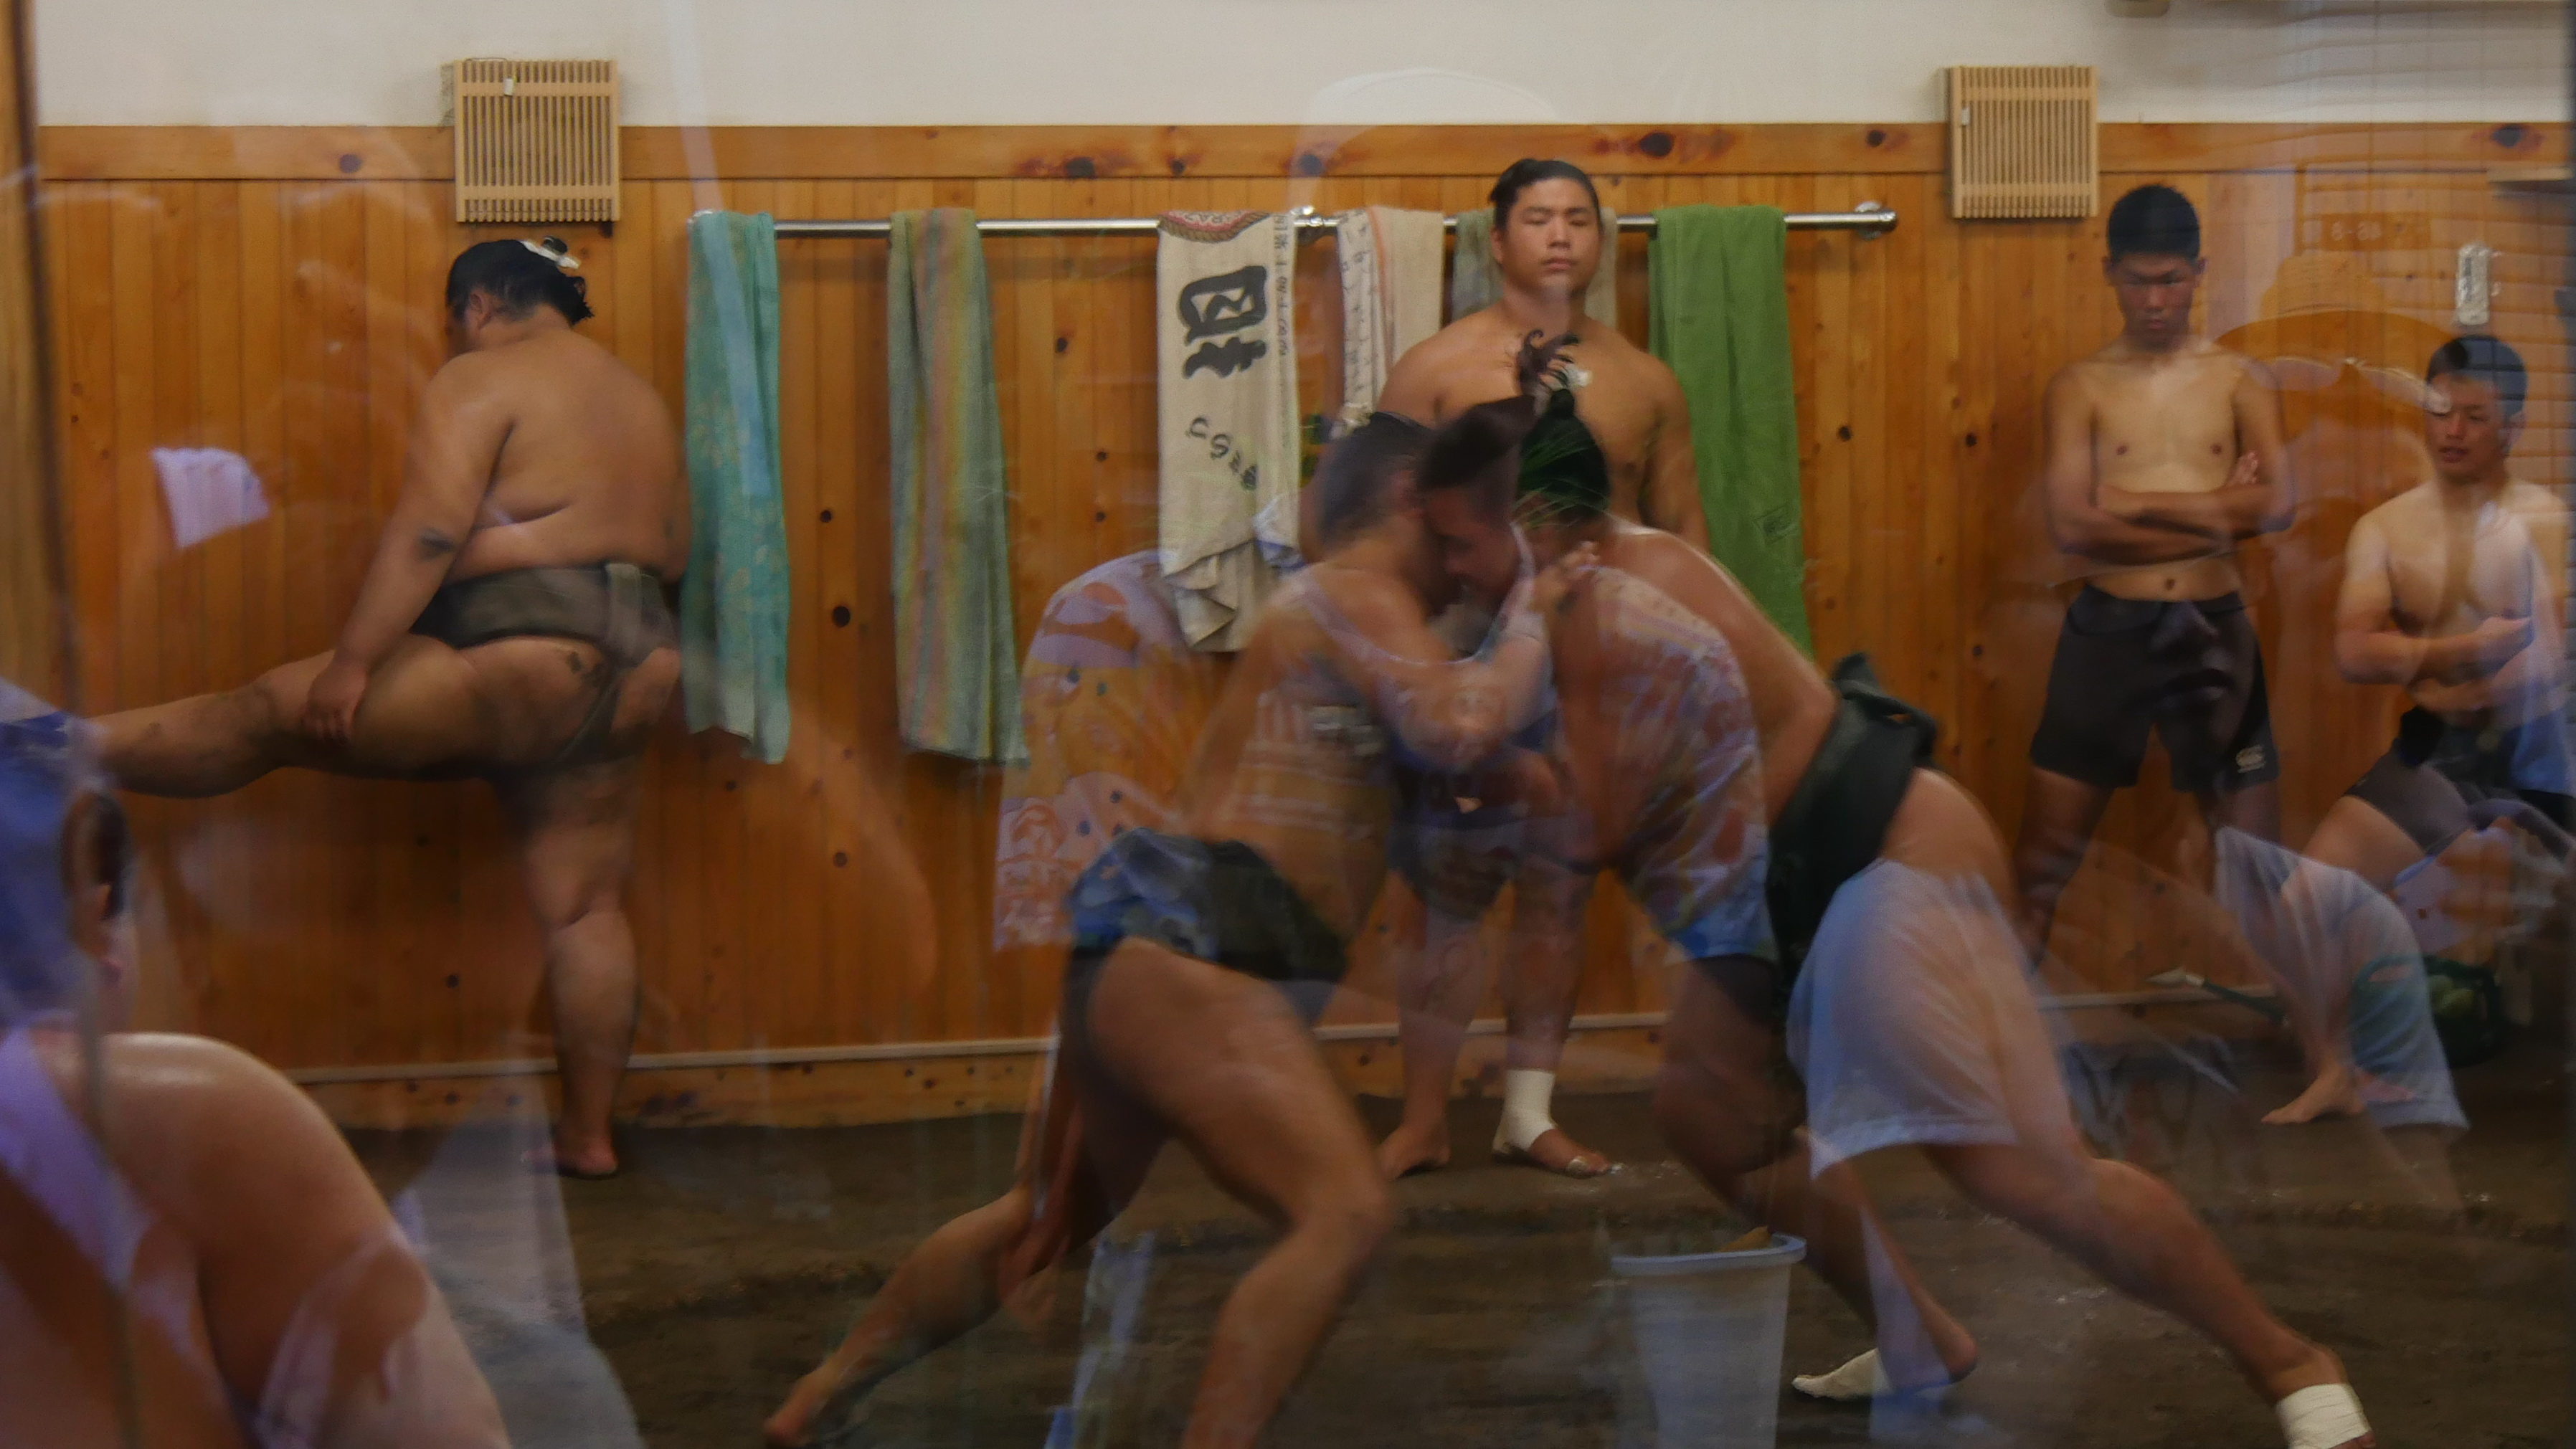
\includegraphics[width=0.9\textwidth]{images/ch01_history/sumo_training.jpg}
\caption{Morning training session at a Tokyo sumo stable, 2014. Junior wrestlers practice under the oyakata's supervision in the keikoba (training ring). Photo: Public domain via Wikimedia Commons.}
\label{fig:sumo_training}
\end{figure}

\subsubsection{The Hierarchy: Sekitori and Wakaisho}

Wrestlers divide into two castes with radically different lived experiences:

\begin{itemize}
\item \textbf{Sekitori} (\japterm{sekitori}{関取}): Wrestlers in the top two divisions (makuuchi and juryo). These are salaried employees of the Japan Sumo Association, earning substantial monthly stipends that increase with rank. Sekitori enjoy private rooms, personal attendants drawn from lower-ranked wrestlers, freedom to marry, the right to wear silk mawashi and elaborate kesho-mawashi during ring-entering ceremonies, and relative autonomy in daily life.
\item \textbf{Wakaisho} (\japterm{wakaisho}{若い衆}): All other wrestlers, comprising the vast majority of stable residents. These men are unsalaried, receiving only small monthly stipends (often around 100,000 yen or roughly \$700 USD). They share cramped sleeping quarters, often sleeping in groups on the floor of common rooms. They perform all stable chores: cooking, cleaning, laundry, and serving as personal attendants to sekitori. They cannot marry without permission, which is rarely granted to anyone below juryo rank.
\end{itemize}

This division is absolute. A wrestler promoted from makushita (the highest unsalaried division) to juryo undergoes an instant transformation in status, moving from shared quarters to a private room, from servant to master. Conversely, demotion from juryo to makushita means loss of salary, privacy, and autonomy—a fall that often precipitates retirement.

\subsubsection{The Daily Schedule}

A typical day at a sumo stable follows an unvarying pattern designed to maximize training intensity while building group cohesion:

\begin{enumerate}
\item \textbf{5:00--6:00 AM}: Wrestlers rise before dawn. Junior wrestlers wake earlier to prepare the training area and begin chores.
\item \textbf{6:00--11:00 AM}: Morning practice (\japterm{keiko}{稽古}) begins. Training occurs on an empty stomach, a practice believed to increase intensity and mental toughness. Sessions last 3--5 hours without breaks, consisting of repetitive drills, practice bouts (\japterm{butsukari-geiko}{ぶつかり稽古}), and full-intensity matches between wrestlers. The oyakata observes, offering corrections and occasionally demonstrating techniques. Higher-ranked wrestlers train first while lower-ranked wrestlers wait their turn, reinforcing hierarchy through every aspect of practice.
\item \textbf{11:00 AM--12:00 PM}: While sekitori bathe and relax, junior wrestlers prepare the first meal of the day.
\item \textbf{12:00--2:00 PM}: The communal meal, centered on \japterm{chanko-nabe}{ちゃんこ鍋}, a protein-rich stew designed to help wrestlers gain weight. Chanko is not a single recipe but a category of hearty stews, often including chicken, fish, tofu, vegetables, and broth, accompanied by rice and side dishes. Junior wrestlers serve sekitori first, eating only after their seniors are satisfied. This meal is enormous, often constituting 3,000--5,000 calories.
\item \textbf{2:00--5:00 PM}: Mandatory nap time. Sleeping after the massive midday meal promotes weight gain and recovery. Sekitori sleep in private rooms while junior wrestlers share common spaces.
\item \textbf{5:00--8:00 PM}: Free time for sekitori; junior wrestlers continue chores, prepare the evening meal, and handle stable maintenance.
\item \textbf{8:00--9:00 PM}: Evening meal, again communal and hierarchical. The meal is substantial but less overwhelming than lunch.
\item \textbf{9:00--10:00 PM}: Wrestlers retire, with junior wrestlers ensuring the stable is clean and secure before sleeping.
\end{enumerate}

This schedule repeats with almost no variation, six days per week, throughout the year except during tournament periods when training gives way to competition. The monotony is intentional, creating a structured environment that minimizes external distractions and focuses attention entirely on sumo.

\subsubsection{The Role of the Okamisan}

The stable master's wife occupies a position of extraordinary authority and responsibility. She manages finances, often controlling all money flowing through the stable including wrestlers' savings. She organizes supporter club functions, dinners with patrons and sponsors, and recruitment efforts. She oversees the kitchen and teaches junior wrestlers basic life skills. In some cases, when an oyakata is in poor health, the okamisan even supervises training.

Her role extends to counseling young wrestlers through personal crises, mediating disputes, and maintaining stable morale. Without an effective okamisan, many stables would struggle to function. This is why marriage is mandatory for stable masters: the institution requires both father and mother figures to operate.

The okamisan's power is informal but pervasive. She cannot hold official rank in the association, but her influence within the stable often rivals or exceeds that of assistant coaches. Former wrestlers' wives bring their own networks and expertise, creating dynasties where sumo knowledge passes through both male and female lines.

\subsection{Economics and Sustainability}

Running a stable is expensive. The oyakata must secure and maintain a physical facility, often in expensive urban areas like Tokyo where land values are exorbitant. He must feed dozens of young men who consume enormous quantities of food. He must pay for medical care, equipment, utilities, transportation to tournaments, and salaries for any staff beyond the wrestlers themselves.

Revenue comes from several sources:

\begin{itemize}
\item \textbf{Association stipends}: The JSA provides financial support to stables, though the amounts are modest relative to operating costs.
\item \textbf{Sekitori salaries shared with the stable}: While sekitori receive salaries directly, they traditionally contribute a portion back to the stable that trained them, particularly for major expenses.
\item \textbf{Tournament bonuses}: When a stable's wrestler wins or performs exceptionally, the stable receives prize money.
\item \textbf{Supporter associations} (\japterm{koen-kai}{後援会}): These are groups of fans and patrons who provide financial support to stables in exchange for access to wrestlers, special events, and social prestige. Wealthy supporters can contribute millions of yen annually, making the cultivation of these relationships essential to stable survival.
\item \textbf{Corporate sponsorships}: Some stables secure sponsorships from businesses seeking association with sumo's traditional prestige.
\item \textbf{Personal wealth}: Many oyakata subsidize their stables from personal funds, particularly in the early years before a stable's wrestlers reach salaried ranks.
\end{itemize}

The economic model is precarious. A stable with no sekitori operates at a loss, dependent entirely on supporter generosity and the oyakata's resources. A stable with multiple high-ranking sekitori can be profitable, but success in the ring is unpredictable. This creates strong incentives to recruit promising young talent and intense pressure to develop them quickly.

The foreign-born wrestler restriction—one per stable—affects economics significantly. Foreign wrestlers, particularly Mongolians, have dominated the top ranks in recent decades. A stable fortunate enough to recruit a successful foreign wrestler gains enormous financial advantage, but the one-per-stable cap prevents any heya from monopolizing foreign talent. This rule, implemented in February 2002, replaced an earlier system allowing two foreigners per stable, reflecting association concerns about foreign dominance.

\subsection{Training Philosophy and Stable Culture}

Not all stables train identically. While the basic structure remains consistent—morning practice, communal meals, hierarchical living arrangements—stable masters develop distinct philosophies that shape their wrestlers' styles and career trajectories.

Some stables emphasize technical precision, drilling specific techniques until they become reflexive. Others prioritize raw physicality, focusing on strength conditioning and aggressive practice bouts. Some oyakata are hands-on, participating actively in daily training; others observe and correct from a distance. These differences create identifiable stable styles: Miyagino stable under Hakuhō was known for technical sophistication and strategic patience; Takasago stable has historically produced powerful, aggressive wrestlers.

The culture extends beyond training to recruitment. Some stables actively scout throughout Japan and internationally, seeking physically gifted teenagers who can be molded into wrestlers. Others rely on family connections, recruiting sons and relatives of former wrestlers. Takamiyama, the first foreign-born wrestler to reach makuuchi, later founded Azumazeki stable and used his Hawaiian connections to recruit Akebono and Musashimaru, both of whom became yokozuna. This pipeline approach—leveraging geographic or social networks to concentrate talent from specific populations—can produce sustained success.

Stable reputation matters enormously for recruitment. A stable that has produced yokozuna or ozeki in recent memory attracts ambitious young recruits who believe that lineage indicates superior training. Conversely, stables in decline struggle to recruit, creating vicious cycles where lack of talent leads to poor tournament performance, which deters future recruits.

\subsection{Famous Stables and Their Legacies}

Certain stables have shaped sumo history through sustained excellence or cultural impact:

\begin{itemize}
\item \textbf{Tatsunami stable}: One of the oldest continuous stables, founded 1876. Produced yokozuna Futabayama (1930s), who achieved an unprecedented 69-bout winning streak that stood for decades as sumo's most legendary record, and Haguroyama, who ended Dewanoumi stable's long dominance. Tatsunami remains active and aligned with Dewanoumi ichimon.
\item \textbf{Takasago stable}: Historically prestigious, produced seven yokozuna including Asashōryū and Asahifuji. Also produced Konishiki, the first non-Japanese ozeki (Hawaiian). In September 2025, Takasago saw three sekitori promotions in a single tournament, the first time this had occurred for any stable since Sadogatake in September 1979, demonstrating its continued competitiveness.
\item \textbf{Miyagino stable}: Home to Hakuhō, arguably the greatest wrestler in sumo history with 45 tournament championships. Hakuhō became stable master in 2021 after acquiring Miyagino elder stock, but the stable was forcibly closed in March 2024 following the Hokuseihō abuse scandal. Its closure exemplifies how quickly institutional prestige can collapse under disciplinary pressure.
\item \textbf{Dewanoumi stable}: Historically dominant in the early 20th century, the stable name became synonymous with sumo excellence and its descendants form the second-largest ichimon. Though the original Dewanoumi stable closed, its lineage persists through affiliated stables.
\item \textbf{Azumazeki stable}: Founded by Takamiyama (the first foreign makuuchi wrestler), became famous for Hawaiian recruitment pipeline that produced yokozuna Akebono and Musashimaru. Demonstrates how a single successful foreign wrestler could transform a stable's trajectory by leveraging ethnic and geographic networks.
\end{itemize}

These stables illustrate how institutional success compounds across generations. A stable that produces a yokozuna gains prestige that attracts recruits, some of whom become champions who eventually return as coaches, perpetuating excellence. Conversely, stables without recent success struggle to break into the elite tier, lacking the reputation needed to recruit top talent.

Table \ref{tab:stable_success} presents success metrics for selected prominent stables, measured by total yokozuna produced (all-time) and current sekitori count (as of 2024).

\begin{table}[h]
\centering
\small
\caption{Success Metrics for Selected Sumo Stables}
\label{tab:stable_success}
\begin{tabular}{lccc}
\toprule
\textbf{Stable} & \textbf{Yokozuna} & \textbf{Status} & \textbf{Ichimon} \\
\midrule
Takasago & 7 & Active & Takasago \\
Tatsunami & 2+ & Active & Dewanoumi \\
Miyagino & 1 (Hakuhō) & Closed 2024 & -- \\
Kokonoe & 3 & Active & Takasago \\
Isegahama & 4 & Active & Isegahama \\
\bottomrule
\end{tabular}
\end{table}

\subsection{The Stable as Data-Generating Institution}

For researchers, the stable system creates both opportunities and complications. On one hand, it provides natural clustering for hierarchical models: wrestlers within a stable share training methods, coaching, dietary practices, and competitive strategies, making stable affiliation a crucial random effect in any outcome model. Stable-level analysis can reveal which training philosophies produce superior results and whether success concentrates due to coaching quality or simply talent recruitment.

On the other hand, the same-stable non-competition rule creates systematic missing data. When estimating wrestler strength using rating systems like Elo or Glicko, we never observe within-stable matchups, which can bias estimates if stable membership correlates with wrestler quality. The missing data is not random: strong stables accumulate strong wrestlers, but those wrestlers never face each other in regulation bouts (except rare playoff scenarios), meaning our most informative potential comparisons remain unobserved.

The foreign wrestler cap also complicates analysis. If Mongolian wrestlers are systematically stronger (as recent tournament results suggest), then stables lucky enough to recruit successful Mongolians enjoy enormous competitive advantages, but each stable can have only one. This creates winner-take-all dynamics at the recruitment stage, where a single high-value foreign recruit can determine a stable's trajectory for a decade.

Finally, the ichimon system introduces political economy considerations. Wrestlers from aligned stables might—consciously or unconsciously—adjust effort when facing opponents from allied clans, particularly in tournaments where outcomes affect promotion decisions. While match-fixing scandals have erupted periodically, the more subtle question is whether factional loyalty creates detectable patterns in bout outcomes even absent overt collusion. These are empirical questions that later chapters will address.

\subsection{Modern Challenges and Evolution}

The stable system faces pressures that would have been unimaginable a century ago. Declining birth rates in Japan mean fewer potential recruits. The sport's grueling demands and hierarchical culture deter many young men who have less brutal career options available. Scandals involving hazing, physical abuse, and financial impropriety have damaged sumo's public image, making parental consent for teenage recruitment harder to obtain.

The 2006 regulatory tightening, while intended to preserve quality by restricting stable ownership to elite former wrestlers, has also created succession crises. Smaller stables without a pipeline of champions struggle to find qualified inheritors, leading to closures and consolidation. The current equilibrium of around 46 stables may represent a new normal, with total stable count unlikely to return to historical peaks absent regulatory reform.

Technological change also affects traditional stable life. Wrestlers now use smartphones, access social media, and maintain public profiles in ways that would have been impossible in earlier eras. This connectivity undermines the total institution model, introducing external influences and comparisons that can destabilize stable hierarchy. Some oyakata have banned phones during training periods; others embrace technology as recruitment and fan engagement tools.

The foreign wrestler debate continues to evolve. Mongolian dominance has prompted periodic calls for tighter restrictions, met by counterarguments that foreign wrestlers have revitalized interest in the sport and that nationalist restrictions betray sumo's claim to be "Japan's national sport" open to all. The citizenship requirement for elder stock means successful foreign wrestlers face a profound choice: remain citizens of their birth countries and retire completely from sumo after their wrestling careers end, or naturalize as Japanese and potentially become stable masters themselves. Hakuhō chose the latter path, renouncing Mongolian citizenship to acquire Miyagino elder stock, though his stable's subsequent closure demonstrates that even full assimilation provides no guarantee of institutional survival.

The stable system has persisted for over two centuries because it solves fundamental problems: how to train athletes in an specialized combat sport, how to organize tournaments among wrestlers of radically different skill levels, how to preserve institutional knowledge across generations, and how to maintain cultural continuity in a society that has otherwise modernized beyond recognition. Whether it will persist another two centuries depends on its ability to adapt to demographic decline, technological disruption, and changing cultural expectations about hierarchy and authority. For now, it remains the indispensable core of professional sumo, shaping every aspect of the sport that any statistical model must account for.

\section{Tournament Structure Evolution}

The modern six-tournament annual schedule crystallized in 1958, replacing earlier irregular patterns:

\begin{table}[h]
\centering
\begin{tabular}{ll}
\toprule
Period & Annual Tournaments \\
\midrule
Pre-1926 & 2 (10 days each) \\
1926--1948 & 2--4 (variable) \\
1949--1957 & 3--5 (11--15 days) \\
1958--present & 6 (15 days each) \\
\bottomrule
\end{tabular}
\caption{Evolution of annual tournament frequency}
\end{table}

Each \japterm{honbasho}{honbasho} (official tournament) follows an identical structure:
\begin{itemize}
\item 15 days of competition
\item One bout per wrestler per day
\item Odd-numbered months (January, March, May, July, September, November)
\item Rotating between Tokyo (3), Osaka (1), Nagoya (1), and Fukuoka (1)
\end{itemize}

This standardization enables consistent statistical analysis across decades while accounting for era-specific effects.
\section{Ranking System}

The \japterm{banzuke}{banzuke} ranking system creates sumo's competitive hierarchy:

\paragraph{Top Division (\japterm{Makuuchi}{makuuchi})}
\begin{itemize}
\item Yokozuna (grand champion): 0--4 active wrestlers
\item Ozeki (champion): 2--5 wrestlers typically
\item Sekiwake: Exactly 2 wrestlers minimum
\item Komusubi: Exactly 2 wrestlers minimum
\item Maegashira: Numbered ranks 1--17 (varies by tournament)
\end{itemize}

\paragraph{Lower Divisions}
\begin{itemize}
\item Juryo (salaried): 28 wrestlers
\item Makushita: 120 wrestlers
\item Sandanme: 180--200 wrestlers
\item Jonidan: 200--250 wrestlers
\item Jonokuchi: 50--90 wrestlers
\end{itemize}

Promotion and demotion follow complex algorithms based on:
\begin{itemize}
\item Win-loss records (8+ wins typically ensures promotion)
\item Current rank
\item Available slots in higher divisions
\item Special criteria for ozeki and yokozuna
\end{itemize}
\section{Technique Classification}

The JSA recognizes 82 official winning techniques (\japterm{kimarite}{kimarite}) plus 5 non-techniques (disqualifications, defaults). These broadly categorize into:

\paragraph{Basic Categories}
\begin{itemize}
\item \textbf{Yotsu-zumo} (yotsu-zumo): Belt/grappling techniques (48 techniques)
\item \textbf{Oshi-zumo} (oshi-zumo): Pushing/thrusting techniques (19 techniques)
\item \textbf{Nage} (nage): Throwing techniques (included in yotsu)
\item \textbf{Special techniques}: Leg trips, dodges, rare maneuvers (15 techniques)
\end{itemize}

Historical kimarite expansion:
\begin{itemize}
\item Pre-1960: 48 recognized techniques
\item 1960: Expanded to 70 techniques
\item 2001: Current 82 techniques established
\end{itemize}
\section{Key Rule Changes Affecting Statistical Analysis}

Several policy changes create natural experiments for analysis:

\paragraph{1958: Six-Tournament System}
Standardized annual schedule enabling consistent performance metrics and career progression patterns.

\paragraph{1972: Makushita Tsukedashi}
Allowed accomplished amateur wrestlers to enter at Makushita 15 or 10, bypassing lower divisions. This created a distinct cohort with different career trajectories.

\paragraph{2003: Abolition of Kōshō System}
Eliminated injury protection that allowed wrestlers to maintain rank while absent. This fundamentally altered injury incentives and risk-taking behavior:
\begin{itemize}
\item Pre-2003: Injured wrestlers could sit out with rank protection
\item Post-2003: Any absence results in automatic demotion
\item Created measurable changes in injury patterns and career longevity
\end{itemize}

\paragraph{2010: Foreign Wrestler Definition Clarification}
Refined rules for naturalized citizens and their stable eligibility, affecting recruitment patterns and competitive balance.
\section{Modern Era Challenges}

Contemporary sumo faces several pressures affecting our data:

\paragraph{Recruitment Crisis}
New wrestler numbers have declined 40\% since 1990, concentrating talent and potentially affecting competitive dynamics.

\paragraph{Internationalization}
Foreign-born wrestlers now dominate upper ranks despite quotas:
\begin{itemize}
\item 67 of 72 yokozuna championships (2004--2024) won by Mongolian wrestlers
\item Increasing technical diversity from international styles
\item Stable recruitment strategies adapted to one-foreign rule
\end{itemize}

\paragraph{Match-Fixing Scandals}
2011 revelations led to tournament cancellation and 23 forced retirements, creating a structural break in our time series and natural experiment for integrity analysis.

\paragraph{Health and Safety Evolution}
Increased medical oversight and concussion protocols since 2018 affect injury reporting and potentially bout outcomes.
\section{Data Implications}

These historical and structural elements create several analytical considerations:

\begin{enumerate}
\item \textbf{Era effects}: Performance metrics must account for rule changes, tournament frequency, and competitive density
\item \textbf{Selection bias}: Foreign wrestler quota creates non-random selection into stables
\item \textbf{Censoring}: Injury absence patterns changed fundamentally in 2003
\item \textbf{Network effects}: Same-stable exclusion creates missing data patterns
\item \textbf{Incentive discontinuities}: Promotion thresholds create non-linear effort incentives
\end{enumerate}

Understanding this historical context is essential for interpreting the statistical patterns we uncover in subsequent chapters. The sport's unique blend of ancient tradition and modern athletics creates a rich but complex data environment requiring careful analytical treatment.

% Chapter references
\printbibliography[heading=subbibliography,title={References}]
% \chapter{Prior Work and Literature Review}

\section{Introduction}

[TO COMPLETE: Overview of existing sumo research across economics, sports science, and medicine]
\section{Economics and Game Theory}

\subsection{The Bubble Effect: Strategic Behavior at 7-7}

[TO COMPLETE: Duggan \& Levitt (2002) analysis of match-fixing]

\subsection{Tournament Theory and Incentives}

[TO COMPLETE: Promotion/demotion thresholds and effort provision]
\section{Sports Science and Performance}

\subsection{Technique Diversity and Success}

[TO COMPLETE: University of Hawaii working paper on versatility]

\subsection{Anthropometric Studies}

[TO COMPLETE: Height, weight, BMI relationships with performance]
\section{Medical and Injury Research}

\subsection{Injury Epidemiology}

[TO COMPLETE: Ota et al. (2023) Hawkes process models]

\subsection{ACL Injuries in Sumo}

[TO COMPLETE: 20% reinjury rate studies]

\subsection{Metabolic Health}

[TO COMPLETE: Energy expenditure, body composition, metabolic syndrome]
\section{Rating Systems and Prediction}

\subsection{Elo-based Approaches}

[TO COMPLETE: Fan-created rating systems]

\subsection{Machine Learning Applications}

[TO COMPLETE: Neural networks, random forests for outcome prediction]
\section{Historical and Cultural Studies}

[TO COMPLETE: Qualitative research on sumo traditions and evolution]
\section{Gaps in the Literature}

[TO COMPLETE: What this book addresses that prior work has not]
% \chapter{Data Infrastructure}

\section{Overview}

[TO COMPLETE: Introduction to the comprehensive data collection effort]
\section{Primary Data Sources}

\subsection{Sumo-API}

[TO COMPLETE: REST API structure, endpoints, data availability 1958-present]

\subsection{Japan Sumo Association}

[TO COMPLETE: Official records, banzuke publications, wrestler profiles]

\subsection{SumoDB}

[TO COMPLETE: Historical database, query capabilities, cross-validation]
\section{Database Design}

\subsection{Schema Architecture}

[TO COMPLETE: Entity-relationship diagram, normalization decisions]

\subsection{Core Tables}

[TO COMPLETE: wrestlers, tournaments, bouts, banzuke, injuries tables]

\subsection{Derived Tables and Views}

[TO COMPLETE: Aggregations, statistics, performance metrics]
\section{Data Collection Pipeline}

\subsection{Bulk Import Process}

[TO COMPLETE: Python scripts, API rate limiting, error handling]

\subsection{Data Validation}

[TO COMPLETE: Consistency checks, cross-source validation, missing data]

\subsection{Update Procedures}

[TO COMPLETE: Tournament-by-tournament updates, real-time integration]
\section{Data Quality and Completeness}

\subsection{Coverage Analysis}

[TO COMPLETE: Bouts by year, missing tournaments, data gaps]

\subsection{Known Limitations}

[TO COMPLETE: Historical data issues, injury reporting gaps, weight snapshots]
\section{Computational Infrastructure}

[TO COMPLETE: Database performance, indexing strategies, query optimization]
\section{Reproducibility}

[TO COMPLETE: Version control, data snapshots, replication instructions]
% \chapter{Measurement: Turning Sumo Into Variables}

\section{Introduction}

[TO COMPLETE: Philosophy of measurement in sports analytics]
\section{Outcome Variables}

\subsection{Bout-Level Outcomes}

[TO COMPLETE: Win/loss, kimarite, match duration]

\subsection{Tournament-Level Outcomes}

[TO COMPLETE: Kachi-koshi, final record, rank change]

\subsection{Career-Level Outcomes}

[TO COMPLETE: Longevity, highest rank achieved, retirement timing]
\section{Wrestler Characteristics}

\subsection{Physical Attributes}

[TO COMPLETE: Height, weight, BMI, time-varying measurement challenges]

\subsection{Geographic and Cultural Variables}

[TO COMPLETE: Shusshin coding, foreign-born classification, regional effects]

\subsection{Training Environment}

[TO COMPLETE: Heya effects, stablemaster influence, training cohorts]
\section{Technique and Style Quantification}

\subsection{Kimarite Frequency Vectors}

[TO COMPLETE: 82-dimensional technique space, normalization approaches]

\subsection{Style Classification}

[TO COMPLETE: Push vs. grapple spectrum, clustering approaches]

\subsection{Technique Diversity Metrics}

[TO COMPLETE: Shannon entropy, Simpson index, versatility measures]

\subsection{Temporal Evolution}

[TO COMPLETE: Technique changes over career, adaptation patterns]
\section{Competition Context}

\subsection{Opponent Strength}

[TO COMPLETE: Rating differentials, head-to-head records, style matchups]

\subsection{Tournament Position}

[TO COMPLETE: Day effects, pressure situations, clinch scenarios]

\subsection{Era and Cohort Effects}

[TO COMPLETE: Rule changes, competitive density, generational shifts]
\section{Injury and Health Proxies}

\subsection{Absence Patterns}

[TO COMPLETE: Kyujo as injury proxy, severity inference]

\subsection{Performance Degradation}

[TO COMPLETE: Post-injury performance, recovery trajectories]
\section{Composite Indices}

[TO COMPLETE: Overall performance rating, dominance scores, consistency metrics]
\section{Measurement Validation}

[TO COMPLETE: Reliability tests, construct validity, predictive validity]
% \chapter{The Sumo Landscape: Descriptive Analysis}

\section{Introduction}

[TO COMPLETE: Overview of 66 years of professional sumo data]
\section{Tournament Evolution}

\subsection{Structural Changes Over Time}

[TO COMPLETE: Number of wrestlers, tournament format changes, division sizes]

\subsection{Competitive Density}

[TO COMPLETE: Win rate distributions, parity measures, dominance periods]
\section{The Kimarite Ecology}

\subsection{Technique Frequency Distributions}

[TO COMPLETE: Most common techniques by era, rare kimarite occurrences]

\subsection{Evolution of Winning Techniques}

[TO COMPLETE: Time series of technique usage, innovation and obsolescence]

\subsection{Division-Specific Patterns}

[TO COMPLETE: Technique differences across skill levels]
\section{Physical Dimensions of Success}

\subsection{Anthropometric Distributions}

[TO COMPLETE: Height, weight, BMI distributions over time]

\subsection{The Size-Success Relationship}

[TO COMPLETE: Optimal physique analysis, non-linear effects]

\subsection{International Comparison}

[TO COMPLETE: Japanese vs. foreign wrestler characteristics]
\section{Geographic Patterns}

\subsection{Domestic Origins}

[TO COMPLETE: Prefecture-level analysis, regional wrestling styles]

\subsection{The Foreign Invasion}

[TO COMPLETE: Timeline of international participation, country-specific success]

\subsection{Migration to Tokyo}

[TO COMPLETE: Stable recruitment patterns, regional talent pipelines]
\section{Stable Dynamics}

\subsection{Heya Performance Rankings}

[TO COMPLETE: Which stables produce champions, consistency over time]

\subsection{Training Philosophy Differences}

[TO COMPLETE: Technical specialization by stable, size/style preferences]

\subsection{The Same-Stable Exclusion Effect}

[TO COMPLETE: Missing matchups, statistical implications]
\section{Career Trajectories}

\subsection{Typical Career Paths}

[TO COMPLETE: Progression speeds, plateau points, decline patterns]

\subsection{Early Success Indicators}

[TO COMPLETE: Predictors of elite achievement from early career]

\subsection{Retirement Patterns}

[TO COMPLETE: Age, rank, injury influences on retirement]
\section{Rank Dynamics}

\subsection{Promotion and Demotion Flows}

[TO COMPLETE: Transition matrices, expected time at each rank]

\subsection{The Ozeki Bottleneck}

[TO COMPLETE: Difficulty of ozeki promotion, survival analysis]

\subsection{Yokozuna Dominance}

[TO COMPLETE: Championship concentration, reign durations]
\section{Injury and Absence Patterns}

[TO COMPLETE: Kyujo frequency, career impact, recovery success rates]

% % Part II: Analysis
% \part{Statistical Analysis}
% \chapter{Statistical Models of Sumo Performance}

\section{Introduction}

[TO COMPLETE: Modeling philosophy, causal vs. predictive goals]
\section{Bout-Level Models}

\subsection{Basic Logistic Regression}

[TO COMPLETE: P(win) as function of wrestler characteristics]

\subsection{Mixed Effects Models}

[TO COMPLETE: Random effects for wrestlers, tournaments, stables]

\begin{equation}
\text{logit}(P(\text{win}_{ijkt})) = \beta_0 + \beta_1 X_{it} + \beta_2 X_{jt} + \alpha_i + \gamma_j + \delta_k + \epsilon_t
\end{equation}

\subsection{Interaction Effects}

[TO COMPLETE: Style matchups, size interactions, experience differentials]

\subsection{Model Diagnostics}

[TO COMPLETE: Residual analysis, influence diagnostics, cross-validation]
\section{Tournament-Level Models}

\subsection{Kachi-koshi Prediction}

[TO COMPLETE: Binary outcome models, threshold effects at 7-7]

\subsection{Win Count Models}

[TO COMPLETE: Poisson, negative binomial, zero-inflated models]

\subsection{Rank Change Models}

[TO COMPLETE: Ordinal regression for promotion/demotion]
\section{Rating Systems}

\subsection{Elo Implementation}

[TO COMPLETE: K-factor selection, initial ratings, performance]

\subsection{Glicko and Uncertainty}

[TO COMPLETE: Rating deviation, activity bonuses, convergence]

\subsection{Custom Sumo Ratings}

[TO COMPLETE: Incorporating kimarite, injuries, tournament importance]

\subsection{Rating Validation}

[TO COMPLETE: Prediction accuracy, calibration, comparison to banzuke]
\section{Career Trajectory Models}

\subsection{Survival Analysis}

[TO COMPLETE: Time to first makuuchi, career length, retirement hazards]

\subsection{Multi-State Models}

[TO COMPLETE: Transitions between ranks, absorbing states]

\subsection{Growth Curve Models}

[TO COMPLETE: Performance trajectories, peak age, decline rates]
\section{Technique Evolution Models}

\subsection{Markov Models for Style Changes}

[TO COMPLETE: Technique transition matrices, steady states]

\subsection{Diversity and Success}

[TO COMPLETE: Entropy as predictor, optimal versatility]
\section{Hierarchical Bayesian Models}

\subsection{Wrestler Ability Estimation}

[TO COMPLETE: Latent ability parameters, shrinkage, posterior distributions]

\subsection{Stable Effects}

[TO COMPLETE: Hierarchical structure, partial pooling]
\section{Machine Learning Approaches}

\subsection{Random Forests}

[TO COMPLETE: Feature importance, out-of-bag error, interpretability]

\subsection{Neural Networks}

[TO COMPLETE: Architecture, training, performance vs. interpretability]

\subsection{Ensemble Methods}

[TO COMPLETE: Model averaging, stacking, super learners]
\section{Model Comparison}

[TO COMPLETE: AIC/BIC, cross-validation, predictive accuracy metrics]
% \chapter{Causality and Natural Experiments}

\section{Introduction}

[TO COMPLETE: Challenges of causal inference in observational sports data]
\section{The Fundamental Problem}

\subsection{Selection Bias}

[TO COMPLETE: Non-random assignment to stables, weight classes, opponents]

\subsection{Confounding}

[TO COMPLETE: Ability, effort, coaching quality as unobservables]

\subsection{Reverse Causality}

[TO COMPLETE: Does success cause weight gain or vice versa?]
\section{Natural Experiment 1: The 2003 Kosho Abolition}

\subsection{Background}

[TO COMPLETE: Injury protection system, moral hazard concerns]

\subsection{Identification Strategy}

[TO COMPLETE: Difference-in-differences, treated vs. control wrestlers]

\subsection{Results}

[TO COMPLETE: Changes in injury rates, risk-taking, career length]

\subsection{Robustness Checks}

[TO COMPLETE: Parallel trends, placebo tests, sensitivity analysis]
\section{Natural Experiment 2: Foreign Wrestler Quota}

\subsection{The 2010 Clarification}

[TO COMPLETE: Rule change details, affected wrestlers]

\subsection{Regression Discontinuity Design}

[TO COMPLETE: Cutoff exploitation, bandwidth selection, fuzzy RD]

\subsection{Effects on Competition}

[TO COMPLETE: Diversity, success rates, stable composition]
\section{The 7-7 Bubble Revisited}

\subsection{Replicating Duggan-Levitt}

[TO COMPLETE: Updated data, original methodology]

\subsection{Post-Scandal Changes}

[TO COMPLETE: 2011 match-fixing scandal as intervention]

\subsection{Machine Learning Detection}

[TO COMPLETE: Anomaly detection, predictive models of corruption]
\section{Instrumental Variables Approaches}

\subsection{Birthplace as Instrument}

[TO COMPLETE: Distance to Tokyo, local wrestling tradition]

\subsection{Birth Order Effects}

[TO COMPLETE: Family pressure, alternative career options]
\section{Panel Data Methods}

\subsection{Fixed Effects Models}

[TO COMPLETE: Wrestler fixed effects, age-period-cohort models]

\subsection{Dynamic Panel Models}

[TO COMPLETE: Lagged performance, Arellano-Bond estimation]
\section{Matching Methods}

\subsection{Propensity Score Matching}

[TO COMPLETE: Foreign vs. domestic wrestlers, injury effects]

\subsection{Coarsened Exact Matching}

[TO COMPLETE: Stable assignment, physique comparisons]
\section{Synthetic Control Methods}

[TO COMPLETE: Individual wrestler interventions, injury impacts]
\section{Limitations and Caveats}

[TO COMPLETE: External validity, SUTVA violations, interpretation bounds]

% % Part III: Advanced Topics
% \part{Advanced Topics}
% \chapter{Injuries and Physical Health}

\section{Introduction}

[TO COMPLETE: The physical toll of professional sumo]
\section{Injury Epidemiology}

\subsection{Prevalence and Incidence}

[TO COMPLETE: 88\% career injury rate, tournament absence patterns]

\subsection{Injury Types and Locations}

[TO COMPLETE: Knee 35-40\%, back 25-30\%, shoulder 15-20\%]

\subsection{Severity Classification}

[TO COMPLETE: Days lost, career-ending vs. minor, chronic vs. acute]
\section{The ACL Crisis}

\subsection{Incidence Rates}

[TO COMPLETE: Primary tears, 20\% reinjury rate analysis]

\subsection{Risk Factors}

[TO COMPLETE: Weight, technique, previous injury, age]

\subsection{Treatment Decisions}

[TO COMPLETE: Surgery vs. conservative, rank considerations]

\subsection{Return to Competition}

[TO COMPLETE: Recovery time, performance post-return, re-injury risk]
\section{Predictive Models of Injury}

\subsection{The Hawkes Process Approach}

[TO COMPLETE: Ota et al. (2023) methodology, self-exciting processes]

\subsection{Machine Learning Predictions}

[TO COMPLETE: Feature engineering, model performance, early warning systems]

\subsection{Individual Risk Profiling}

[TO COMPLETE: Personalized injury probability, prevention strategies]
\section{Body Composition and Metabolic Health}

\subsection{Extreme Anthropometry}

[TO COMPLETE: BMI 36.5 average, health implications]

\subsection{Energy Balance}

[TO COMPLETE: 4200-6500 kcal/day expenditure, DLW studies]

\subsection{Metabolic Syndrome}

[TO COMPLETE: Diabetes, hypertension, dyslipidemia prevalence]

\subsection{Body Composition Changes}

[TO COMPLETE: Fat vs. muscle gain, career evolution]
\section{Cardiovascular Health}

\subsection{Sleep Apnea}

[TO COMPLETE: 25-30\% prevalence, performance impacts]

\subsection{Cardiac Events}

[TO COMPLETE: OHCA on tournament days, stress factors]

\subsection{Long-term Cardiovascular Risk}

[TO COMPLETE: Post-retirement health, life expectancy]
\section{Injury Prevention Strategies}

\subsection{Training Modifications}

[TO COMPLETE: Load management, technique training, flexibility]

\subsection{Nutritional Interventions}

[TO COMPLETE: Controlled weight gain, supplementation]

\subsection{Medical Monitoring}

[TO COMPLETE: Regular screening, biomarkers, imaging]
\section{The Kosho System and Moral Hazard}

[TO COMPLETE: Pre-2003 injury protection, behavioral changes post-abolition]
\section{Career Impact of Injuries}

\subsection{Rank Trajectories}

[TO COMPLETE: Demotion during recovery, comeback success rates]

\subsection{Retirement Decisions}

[TO COMPLETE: Injury as retirement trigger, survival analysis]

\subsection{Financial Implications}

[TO COMPLETE: Salary loss, career earnings impact]
\section{Comparative Sports Medicine}

[TO COMPLETE: Injury rates vs. other combat sports, unique sumo factors]
\section{Future Directions}

[TO COMPLETE: Wearable technology, biomechanical analysis, prevention programs]
% \chapter{Prediction and Forecasting}

\section{Introduction}

[TO COMPLETE: Predictive modeling in sports, evaluation without gambling]
\section{Short-term Prediction: Next Bout}

\subsection{Feature Engineering}

[TO COMPLETE: Recent form, head-to-head, physical matchup, tournament situation]

\subsection{Model Selection}

[TO COMPLETE: Logistic regression baseline, ensemble methods, neural networks]

\subsection{Real-time Prediction}

[TO COMPLETE: Live tournament predictions, updating with new information]
\section{Medium-term: Tournament Outcomes}

\subsection{Kachi-koshi Probability}

[TO COMPLETE: After day 1, 5, 10 predictions, uncertainty quantification]

\subsection{Championship Prediction}

[TO COMPLETE: Yusho probability, playoff scenarios]

\subsection{Rank Change Forecasting}

[TO COMPLETE: Expected promotion/demotion, banzuke prediction]
\section{Long-term: Career Trajectories}

\subsection{Breakthrough Prediction}

[TO COMPLETE: Time to makuuchi, ozeki probability, yokozuna potential]

\subsection{Career Length Forecasting}

[TO COMPLETE: Expected remaining tournaments, retirement probability]

\subsection{Decline Detection}

[TO COMPLETE: Peak identification, performance degradation patterns]
\section{Rating System Performance}

\subsection{Elo Accuracy}

[TO COMPLETE: Calibration plots, Brier scores, ROC curves]

\subsection{Glicko Improvements}

[TO COMPLETE: Uncertainty benefits, activity adjustments]

\subsection{Hybrid Models}

[TO COMPLETE: Combining ratings with other features]
\section{Technique-based Prediction}

\subsection{Style Matchup Models}

[TO COMPLETE: Push vs. grapple advantages, specific technique success]

\subsection{Adaptation Prediction}

[TO COMPLETE: Technique evolution, counter-strategy development]
\section{Injury Prediction}

\subsection{Next Injury Probability}

[TO COMPLETE: Individual risk scores, temporal dynamics]

\subsection{Severity Prediction}

[TO COMPLETE: Minor vs. career-threatening, recovery time estimation]
\section{Ensemble and Meta-learning}

\subsection{Model Stacking}

[TO COMPLETE: Combining diverse models, weighted averaging]

\subsection{Online Learning}

[TO COMPLETE: Adaptive models, concept drift, tournament-specific tuning]
\section{Prediction Evaluation}

\subsection{Scoring Rules}

[TO COMPLETE: Log loss, Brier score, calibration metrics]

\subsection{Economic Value}

[TO COMPLETE: Decision-theoretic evaluation, without gambling implications]

\subsection{Comparative Performance}

[TO COMPLETE: vs. rankings, vs. public prediction, vs. random]
\section{Uncertainty Quantification}

\subsection{Prediction Intervals}

[TO COMPLETE: Bootstrapping, Bayesian credible intervals]

\subsection{Calibration Analysis}

[TO COMPLETE: Reliability diagrams, isotonic regression]
\section{Feature Importance and Interpretability}

\subsection{SHAP Values}

[TO COMPLETE: Individual prediction explanation, global importance]

\subsection{Ablation Studies}

[TO COMPLETE: Removing features, marginal contribution]
\section{Temporal Validation}

[TO COMPLETE: Rolling window, expanding window, tournament-by-tournament]
\section{Case Studies in Prediction}

[TO COMPLETE: Specific tournament predictions, upset analysis, model failures]
% \chapter{Case Studies in Sumo Excellence}

\section{Introduction}

[TO COMPLETE: Individual stories illuminating statistical patterns]
\section{The Yokozuna Archetypes}

\subsection{The Dominant Force: Hakuho}

[TO COMPLETE: 45 championships, statistical dominance, longevity factors]

\subsection{The Technician: Kakuryu}

[TO COMPLETE: Versatility metrics, adaptation over career]

\subsection{The Injury Warrior: Terunofuji}

[TO COMPLETE: Comeback from Jonidan, injury management, second peak]
\section{Size and Success Stories}

\subsection{The Giants: Akebono and Musashimaru}

[TO COMPLETE: Maximum size advantage, technique limitations, health costs]

\subsection{The David: Mainoumi}

[TO COMPLETE: Success despite size disadvantage, technique diversity necessity]

\subsection{The Optimal Build: Asashoryu}

[TO COMPLETE: Power-to-weight ratio, speed advantage, complete package]
\section{International Pioneers}

\subsection{The Hawaiian Revolution}

[TO COMPLETE: Takamiyama to Akebono, cultural adaptation, training differences]

\subsection{The Mongolian Dynasty}

[TO COMPLETE: Technical innovation, hunger for success, domination statistics]

\subsection{The European Experiment}

[TO COMPLETE: Baruto, Tochinoshin, different body types and styles]
\section{Technique Specialists}

\subsection{The Ultimate Pusher: Akebono}

[TO COMPLETE: Oshi-zumo perfection, kimarite concentration]

\subsection{The Belt Master: Asashoryu}

[TO COMPLETE: Yotsu-zumo excellence, grip strength advantage]

\subsection{The Innovator: Ura}

[TO COMPLETE: Rare technique usage, unpredictability as strategy]
\section{Career Trajectory Anomalies}

\subsection{The Rocket: Onosato}

[TO COMPLETE: Fastest rise to yokozuna, early indicators, sustainability]

\subsection{The Late Bloomer: Takatoriki}

[TO COMPLETE: Delayed success, persistence, peak timing]

\subsection{The Plateau: Kotooshu}

[TO COMPLETE: Ozeki struggles, inability to break through, consistency vs. excellence]
\section{Stable Success Stories}

\subsection{The Kokonoe Dynasty}

[TO COMPLETE: Multiple yokozuna, training methods, recruitment]

\subsection{The Isegahama Renaissance}

[TO COMPLETE: Terunofuji and Harumafuji, Mongolian connection]

\subsection{The Small Stable Miracle}

[TO COMPLETE: Success despite limited resources, individual attention benefits]
\section{Injury and Redemption}

\subsection{The ACL Survivors}

[TO COMPLETE: Successful returns, technique adaptations, career modifications]

\subsection{The Chronic Warriors}

[TO COMPLETE: Managing persistent injuries, strategic absences]
\section{The 7-7 Specialists}

\subsection{Statistical Anomalies}

[TO COMPLETE: Wrestlers with unusual 8-7 frequencies, clutch performance]

\subsection{The Bubble Riders}

[TO COMPLETE: Career patterns around rank thresholds]
\section{Retirement Decisions}

\subsection{The Perfect Exit: Chiyonofuji}

[TO COMPLETE: Timing, legacy preservation, post-career success]

\subsection{The Forced Farewell: Asashoryu}

[TO COMPLETE: Scandal, premature end, what-if scenarios]

\subsection{The Lingerer: Various Examples}

[TO COMPLETE: Staying too long, rank preservation, financial motivations]
\section{Statistical Outliers}

\subsection{The Consistency King}

[TO COMPLETE: Lowest variance in performance, reliability metrics]

\subsection{The Chaos Agent}

[TO COMPLETE: Highest upset rate, giant-killer profile]

\subsection{The Specialist}

[TO COMPLETE: Dominance against specific opponents/styles]
\section{Lessons from the Data}

[TO COMPLETE: Common patterns, success factors, predictive indicators]
% \chapter{Where the Data Ends: Future Research}

\section{Introduction}

[TO COMPLETE: Limitations of current data, unexplored territories]
\section{Data We Don't Have}

\subsection{Training Data}

[TO COMPLETE: Keiko intensity, practice bouts, morning training routines]

\subsection{Physiological Measurements}

[TO COMPLETE: VO2 max, muscle composition, hormone levels, sleep quality]

\subsection{Psychological Factors}

[TO COMPLETE: Mental health, motivation, pressure handling, personality]

\subsection{Nutritional Details}

[TO COMPLETE: Actual caloric intake, meal timing, supplementation]

\subsection{Social Dynamics}

[TO COMPLETE: Stable relationships, mentorship quality, hazing effects]
\section{Technological Opportunities}

\subsection{Computer Vision}

[TO COMPLETE: Automated kimarite classification, stance analysis, movement patterns]

\subsection{Wearable Sensors}

[TO COMPLETE: Accelerometers, force platforms, real-time biomechanics]

\subsection{Biometric Monitoring}

[TO COMPLETE: Heart rate variability, recovery metrics, stress indicators]

\subsection{Motion Capture}

[TO COMPLETE: 3D movement analysis, technique optimization, injury prevention]
\section{Advanced Statistical Methods}

\subsection{Deep Learning Applications}

[TO COMPLETE: Video analysis, pattern recognition, complex interactions]

\subsection{Causal Machine Learning}

[TO COMPLETE: Heterogeneous treatment effects, optimal policy learning]

\subsection{Network Analysis}

[TO COMPLETE: Wrestler relationships, influence propagation, strategic networks]

\subsection{Topological Data Analysis}

[TO COMPLETE: Shape of technique space, performance manifolds]
\section{Unexplored Research Questions}

\subsection{Optimal Tournament Design}

[TO COMPLETE: Schedule effects, fatigue management, fairness optimization]

\subsection{Recruitment Optimization}

[TO COMPLETE: Talent identification, development pathways, resource allocation]

\subsection{Injury Prevention Programs}

[TO COMPLETE: Personalized training, load management, early intervention]

\subsection{Post-Career Health}

[TO COMPLETE: Long-term outcomes, life expectancy, quality of life]
\section{Cross-Sport Comparisons}

\subsection{Combat Sports Analysis}

[TO COMPLETE: MMA, judo, wrestling parallels, technique transfer]

\subsection{Size-Dependent Sports}

[TO COMPLETE: NFL linemen, rugby forwards, weightlifting]

\subsection{Traditional vs. Modern Training}

[TO COMPLETE: Eastern vs. Western approaches, evolution of methods]
\section{Economic Research}

\subsection{Labor Market Analysis}

[TO COMPLETE: Career earnings, outside options, retirement timing]

\subsection{Tournament Incentives}

[TO COMPLETE: Prize structure optimization, effort provision]

\subsection{Stable Economics}

[TO COMPLETE: Resource allocation, recruitment ROI, training investments]
\section{Cultural and Social Research}

\subsection{Globalization Effects}

[TO COMPLETE: Cultural exchange, technique diffusion, fan demographics]

\subsection{Media and Public Perception}

[TO COMPLETE: Narrative effects, star creation, scandal impacts]

\subsection{Gender and Sumo}

[TO COMPLETE: Women's amateur sumo, cultural barriers, future possibilities]
\section{Policy Implications}

\subsection{Health and Safety Regulations}

[TO COMPLETE: Weight limits, concussion protocols, mandatory rest]

\subsection{Competition Structure}

[TO COMPLETE: Division size, tournament frequency, ranking system]

\subsection{International Development}

[TO COMPLETE: Olympic inclusion, global expansion, rule standardization]
\section{Methodological Advances Needed}

\subsection{Missing Data Methods}

[TO COMPLETE: Injury under-reporting, selection bias, censoring]

\subsection{Multilevel Modeling}

[TO COMPLETE: Bout-day-tournament-career hierarchies]

\subsection{Computational Challenges}

[TO COMPLETE: Big data infrastructure, real-time processing, distributed computing]
\section{Call for Collaboration}

[TO COMPLETE: Data sharing protocols, research partnerships, open science]
\section{The Next Decade}

[TO COMPLETE: Predictions for sumo evolution, research priorities, potential breakthroughs]

% Appendices (stay in main matter for proper numbering)
\part{Appendices}
\appendix
\chapter{Data Dictionary}

\section{Database Schema}

\subsection{wrestlers Table}
\begin{longtable}{llp{7cm}}
\toprule
Field & Type & Description \\
\midrule
\endhead
id & INTEGER & Unique wrestler identifier \\
shikona & TEXT & Ring name (may change over career) \\
real\_name & TEXT & Birth name \\
birth\_date & DATE & Date of birth \\
debut\_date & DATE & Professional debut date \\
retirement\_date & DATE & Retirement date (NULL if active) \\
height\_cm & INTEGER & Height in centimeters \\
weight\_kg & INTEGER & Weight in kilograms \\
shusshin & TEXT & Birthplace/origin \\
heya & TEXT & Stable affiliation \\
foreign\_born & BOOLEAN & True if born outside Japan \\
\bottomrule
\end{longtable}

\subsection{tournaments Table}
\begin{longtable}{llp{7cm}}
\toprule
Field & Type & Description \\
\midrule
\endhead
id & TEXT & Tournament ID (YYYYMM format) \\
year & INTEGER & Tournament year \\
month & INTEGER & Tournament month (1,3,5,7,9,11) \\
location & TEXT & City (Tokyo, Osaka, Nagoya, Fukuoka) \\
start\_date & DATE & First day of tournament \\
end\_date & DATE & Final day of tournament \\
\bottomrule
\end{longtable}

\subsection{bouts Table}
\begin{longtable}{llp{7cm}}
\toprule
Field & Type & Description \\
\midrule
\endhead
id & INTEGER & Unique bout identifier \\
tournament\_id & TEXT & Foreign key to tournaments \\
day & INTEGER & Day of tournament (1-15) \\
division & TEXT & Competition division \\
east\_wrestler\_id & INTEGER & Eastern wrestler ID \\
west\_wrestler\_id & INTEGER & Western wrestler ID \\
winner\_id & INTEGER & Winner's ID \\
kimarite & TEXT & Winning technique \\
match\_time\_seconds & INTEGER & Duration in seconds \\
\bottomrule
\end{longtable}

\subsection{banzuke Table}
\begin{longtable}{llp{7cm}}
\toprule
Field & Type & Description \\
\midrule
\endhead
tournament\_id & TEXT & Foreign key to tournaments \\
wrestler\_id & INTEGER & Foreign key to wrestlers \\
division & TEXT & Division name \\
rank & TEXT & Rank designation (Y, O, S, K, M1-17, J1-14) \\
rank\_number & INTEGER & Numeric rank for ordering \\
east\_west & TEXT & East or West designation \\
\bottomrule
\end{longtable}

\section{Variable Definitions}

\subsection{Derived Variables}

\textbf{win\_rate}: Total wins divided by total bouts (wins + losses)

\textbf{kachi\_koshi}: Binary indicator for achieving winning record (8+ wins)

\textbf{make\_koshi}: Binary indicator for losing record (8+ losses)

\textbf{career\_length}: Years from debut\_date to retirement\_date or current date

\textbf{bmi}: weight\_kg / (height\_cm/100)\^{}2

\textbf{push\_ratio}: Proportion of wins by pushing techniques

\textbf{technique\_diversity}: Shannon entropy of kimarite distribution

\textbf{kyujo\_rate}: Proportion of tournaments with absences

\section{Division Codes}

\begin{tabular}{ll}
\toprule
Code & Division Name \\
\midrule
Y & Yokozuna \\
O & Ozeki \\
S & Sekiwake \\
K & Komusubi \\
M & Maegashira \\
J & Juryo \\
Ms & Makushita \\
Sd & Sandanme \\
Jd & Jonidan \\
Jk & Jonokuchi \\
\bottomrule
\end{tabular}

\section{Missing Data Codes}

\begin{tabular}{ll}
\toprule
Code & Meaning \\
\midrule
NULL & Value unknown or not applicable \\
0 & Confirmed zero/absent \\
-1 & Not yet occurred (future event) \\
-999 & Error or invalid data \\
\bottomrule
\end{tabular}

\section{Data Quality Flags}

[TO COMPLETE: Reliability indicators, source verification, imputation flags]
\chapter{Complete Kimarite Catalog}

\section{Introduction}

[TO COMPLETE: All 82 official winning techniques plus 5 non-techniques]

\section{Basic Techniques (Kihon-waza)}

\subsection{Push/Thrust Techniques (Oshi-waza)}

\begin{longtable}{lllr}
\toprule
Technique & Japanese & Description & Frequency \\
\midrule
\endhead
oshidashi & oshidashi & Push out & 15.2\% \\
oshitaoshi & oshitaoshi & Push down & 8.1\% \\
tsukidashi & tsukidashi & Thrust out & 3.4\% \\
tsukitaoshi & tsukitaoshi & Thrust down & 1.8\% \\
hatakikomi & hatakikomi & Slap down & 6.7\% \\
\bottomrule
\end{longtable}

[TO COMPLETE: All push techniques with descriptions and historical frequencies]

\subsection{Grappling Techniques (Yotsu-waza)}

\begin{longtable}{lllr}
\toprule
Technique & Japanese & Description & Frequency \\
\midrule
\endhead
yorikiri & yorikiri & Force out & 32.1\% \\
uwatenage & uwatenage & Overarm throw & 4.2\% \\
shitatenage & shitatenage & Underarm throw & 2.8\% \\
kotenage & kotenage & Arm throw & 1.6\% \\
sukuinage & sukuinage & Scooping throw & 1.3\% \\
\bottomrule
\end{longtable}

[TO COMPLETE: All grappling techniques]

\section{Special Techniques (Tokushu-waza)}

\subsection{Leg Techniques (Ashi-waza)}

[TO COMPLETE: All leg-based techniques]

\subsection{Twisting Techniques (Hineri-waza)}

[TO COMPLETE: All twisting/turning techniques]

\subsection{Lifting Techniques (Tsuridashi-waza)}

[TO COMPLETE: All lifting techniques]

\section{Rare Techniques}

\subsection{Historical Usage}

[TO COMPLETE: Techniques that were more common in earlier eras]

\subsection{Modern Rarities}

[TO COMPLETE: Techniques rarely seen in contemporary sumo]

\subsection{One-Off Techniques}

[TO COMPLETE: Techniques used only a few times in recorded history]

\section{Non-Techniques (Hi-kimarite)}

\begin{longtable}{lll}
\toprule
Non-technique & Japanese & Description \\
\midrule
hansoku & hansoku & Foul (illegal move) \\
koshikudake & koshikudake & Collapse without contact \\
fumidashi & fumidashi & Step out \\
isamiashi & isamiashi & Overeager step out \\
tottari & tottari & Arm bar throw \\
\bottomrule
\end{longtable}

\section{Technical Analysis}

\subsection{Technique Effectiveness}

[TO COMPLETE: Win rates by technique, situational effectiveness]

\subsection{Evolution Over Time}

[TO COMPLETE: How technique frequencies have changed 1958-2024]

\subsection{Style Correlations}

[TO COMPLETE: Which techniques correlate with body type, origin, stable]

\section{Disputed Decisions}

[TO COMPLETE: Controversial kimarite calls, video review impacts]

\section{Training and Teaching}

[TO COMPLETE: Which techniques are taught first, difficulty progression]
\chapter{Code Repository and Reproducibility}

\section{Repository Structure}

[TO COMPLETE: GitHub repository layout]

\section{Installation and Setup}

\subsection{System Requirements}

\begin{itemize}
\item Python 3.8+ with packages: pandas, numpy, sqlite3, requests
\item SQLite 3.35+
\item LaTeX distribution (TeX Live recommended)
\item R 4.0+ (optional, for some analyses)
\end{itemize}

\subsection{Database Setup}

\begin{lstlisting}[language=bash]
cd database/
sqlite3 sumo.db < setup.sql
python bulk_import.py
\end{lstlisting}

\subsection{Analysis Environment}

[TO COMPLETE: Jupyter notebook setup, package versions, environment files]

\section{Data Collection Scripts}

\subsection{bulk\_import.py}

[TO COMPLETE: Main data collection script documentation]

\subsection{API Integration}

[TO COMPLETE: Sumo-API wrapper functions, rate limiting, error handling]

\subsection{Data Validation}

[TO COMPLETE: Consistency checks, cross-source validation]

\section{Analysis Code}

\subsection{Statistical Models}

[TO COMPLETE: Model fitting scripts, validation procedures]

\subsection{Visualization}

[TO COMPLETE: Figure generation code, plot styling]

\subsection{Performance Metrics}

[TO COMPLETE: Rating calculation, prediction evaluation]

\section{Reproducibility Checklist}

\begin{enumerate}
\item Clone repository: \texttt{git clone [URL]}
\item Install dependencies: \texttt{pip install -r requirements.txt}
\item Run data collection: \texttt{python database/bulk\_import.py}
\item Execute analyses: \texttt{python analysis/run\_all.py}
\item Generate figures: \texttt{python figures/generate\_all.py}
\item Compile book: \texttt{pdflatex main.tex}
\end{enumerate}

\section{Data Versioning}

[TO COMPLETE: Data snapshot management, version control for large files]

\section{Testing}

\subsection{Unit Tests}

[TO COMPLETE: Model validation, data integrity tests]

\subsection{Integration Tests}

[TO COMPLETE: End-to-end pipeline validation]

\section{Documentation}

[TO COMPLETE: Function documentation, API reference, tutorial notebooks]

\section{License and Attribution}

[TO COMPLETE: Open source license, data source attribution, citation requirements]
\chapter{Statistical Methods and Model Details}

\section{Model Specifications}

\subsection{Mixed Effects Logistic Regression}

The primary bout outcome model is specified as:

\begin{align}
\text{logit}(P(Y_{ijkt} = 1)) &= \beta_0 + \boldsymbol{\beta}_1^T \mathbf{X}_{it} + \boldsymbol{\beta}_2^T \mathbf{X}_{jt} \\
&\quad + \boldsymbol{\beta}_3^T \mathbf{Z}_{kt} + \alpha_i + \gamma_j + \delta_k + \epsilon_t
\end{align}

where:
\begin{itemize}
\item $Y_{ijkt} = 1$ if wrestler $i$ beats wrestler $j$ in tournament $k$ on day $t$
\item $\mathbf{X}_{it}$ = wrestler $i$'s characteristics at time $t$
\item $\mathbf{Z}_{kt}$ = tournament/context variables
\item $\alpha_i \sim N(0, \sigma_{\alpha}^2)$ = wrestler random effects
\item $\gamma_j \sim N(0, \sigma_{\gamma}^2)$ = opponent random effects  
\item $\delta_k \sim N(0, \sigma_{\delta}^2)$ = tournament random effects
\item $\epsilon_t \sim N(0, \sigma_{\epsilon}^2)$ = day effects
\end{itemize}

\subsection{Survival Models for Career Analysis}

For career longevity analysis, we employ Cox proportional hazards models:

\begin{equation}
h(t|\mathbf{X}) = h_0(t) \exp(\boldsymbol{\beta}^T \mathbf{X})
\end{equation}

With competing risks framework for different retirement types:
\begin{itemize}
\item Voluntary retirement
\item Forced retirement (injury)
\item Demotion-induced retirement
\end{itemize}

\subsection{Rating System Mathematics}

\subsubsection{Elo System}

Updates follow:
\begin{align}
R_{i,new} &= R_{i,old} + K \cdot (S_i - E_i) \\
E_i &= \frac{1}{1 + 10^{(R_j - R_i)/400}}
\end{align}

where $K$ varies by division and experience:
\begin{equation}
K = \begin{cases}
40 & \text{if new wrestler (first 10 tournaments)} \\
32 & \text{if makuuchi/juryo} \\
24 & \text{if lower divisions}
\end{cases}
\end{equation}

\subsubsection{Glicko System}

Rating updates incorporate uncertainty (rating deviation):

\begin{align}
\phi_{new}^2 &= \frac{1}{\frac{1}{\phi_{old}^2 + \sigma^2} + \frac{1}{v}} \\
\mu_{new} &= \mu_{old} + \phi_{new}^2 \sum_j \frac{g(\phi_j)(s_j - E(\mu, \mu_j, \phi_j))}{\sigma^2}
\end{align}

\section{Estimation Methods}

\subsection{Maximum Likelihood}

For logistic regression models, we maximize:

\begin{equation}
\ell(\boldsymbol{\beta}) = \sum_{i=1}^n \left[ y_i \log p_i + (1-y_i) \log(1-p_i) \right]
\end{equation}

\subsection{Bayesian Estimation}

Hierarchical models estimated using MCMC with priors:

\begin{align}
\boldsymbol{\beta} &\sim N(\mathbf{0}, \tau^2 \mathbf{I}) \\
\sigma_{\alpha}^2 &\sim \text{InvGamma}(a, b) \\
\tau^2 &\sim \text{InvGamma}(c, d)
\end{align}

\subsection{Cross-Validation Procedures}

Time series cross-validation using expanding windows:
\begin{itemize}
\item Training: Tournaments 1 to $t$
\item Testing: Tournament $t+1$
\item Advance $t$ and repeat
\end{itemize}

\section{Model Diagnostics}

\subsection{Residual Analysis}

Pearson residuals for logistic models:
\begin{equation}
r_i = \frac{y_i - \hat{p}_i}{\sqrt{\hat{p}_i(1-\hat{p}_i)}}
\end{equation}

\subsection{Influential Observations}

Cook's distance and DFBETAS for outlier detection.

\subsection{Goodness of Fit}

\begin{itemize}
\item Hosmer-Lemeshow test
\item Calibration plots
\item ROC curves and AUC
\end{itemize}

\section{Prediction Evaluation Metrics}

\subsection{Scoring Rules}

Brier Score:
\begin{equation}
BS = \frac{1}{N} \sum_{i=1}^N (p_i - y_i)^2
\end{equation}

Log Loss:
\begin{equation}
LL = -\frac{1}{N} \sum_{i=1}^N [y_i \log p_i + (1-y_i) \log(1-p_i)]
\end{equation}

\subsection{Calibration Metrics}

Expected Calibration Error (ECE):
\begin{equation}
ECE = \sum_{m=1}^M \frac{|B_m|}{n} |\text{acc}(B_m) - \text{conf}(B_m)|
\end{equation}

\section{Computational Details}

\subsection{Software and Packages}

\begin{itemize}
\item Python: scikit-learn, statsmodels, lifelines
\item R: lme4, survival, rms
\item Stan: Bayesian inference
\item SQLite: Data storage and querying
\end{itemize}

\subsection{Convergence Diagnostics}

For MCMC chains:
\begin{itemize}
\item $\hat{R}$ statistic (Gelman-Rubin)
\item Effective sample size
\item Trace plots
\end{itemize}

\subsection{Computational Complexity}

[TO COMPLETE: Runtime analysis, memory requirements, scalability]

\section{Bootstrap and Resampling}

\subsection{Confidence Intervals}

Percentile method for non-parametric CIs:
\begin{equation}
CI_{1-\alpha} = [\hat{\theta}_{\alpha/2}, \hat{\theta}_{1-\alpha/2}]
\end{equation}

\subsection{Bias Correction}

$BC_a$ method for skewed distributions.

\section{Multiple Testing Corrections}

Benjamini-Hochberg procedure for FDR control:
\begin{equation}
\alpha_{BH} = \frac{i}{m} \cdot \alpha
\end{equation}

\section{Power Analysis}

[TO COMPLETE: Sample size calculations, effect size detection]

\section{Sensitivity Analysis}

[TO COMPLETE: Robustness to model assumptions, prior sensitivity]

% Back matter
\backmatter

% Bibliography
\printbibliography[heading=bibintoc,title={References}]

% Index
\printindex

\end{document}